\documentclass [twocolumn]{article}

\title{Low dose vita-ray exposure does not enhance reaction times}
\author{J. Logan Howlett, Ann Marie, R. L. Drake-Eisman, S. Summers, and K. A. Pryde\thanks{Charles Xavier School for Gifted Youngsters, Salem Center, NY 10560}}
\date{\today}

\usepackage{amsmath,amssymb,amsfonts}
\usepackage{siunitx}
\sisetup{separate-uncertainty=true}
\DeclareSIUnit\xavier{X}
\usepackage{fancyref}
\usepackage{graphicx}
\usepackage{listings}
\lstset{basicstyle=\ttfamily}
\usepackage{hyperref}
\usepackage[dvipsnames]{xcolor}
\hypersetup{
  colorlinks=true,
  linkcolor=violet,
  urlcolor=blue,
  citecolor=blue}

\usepackage{lineno}
\usepackage{natbib}
\bibliographystyle{jeb}

\begin{document}
\maketitle

\begin{abstract}
This paper refutes previous studies of the effect of low-dose vita-ray exposure on non-mutant humans.  Previous studies were not double-blind and suffer from extensive pseudoreplication and cherry picking of data in favor of sponsoring commercial interests.  In this double-blind study, no impact of vita-ray exposure was discerned. 
\end{abstract}

\maketitle

\section{Introduction}
Motivated by military needs, methods of enhancing both reflexes and reaction times using vita-ray exposure have been the subject of active research since at least the 1940s.  Widespread interest in such improvements and therapeutic applications led to a post-war proliferation of both government-sponsored research and private sector commercial interests based on this body of research.  In 2010, private-sector interests stemming from vita-ray equipment were worth \$1.1 billion.  

The seminal study of vita-ray exposure, \citet{lensherr1941enhancement}, irradiated a single male test subject with 1.2 teraxaviers (\si{\tera\xavier}) of vita-rays and reported “improved reflexes and reaction times and greatly improved strength.”  They did not report measures of any of reflexes, response time, or strength before the treatment; nor did they separate the effects of vita-ray exposure from those of the concurrent OSS training received by the one test subject.  Subsequent studies also failed to adequately control for confounding effects, used inadequate numbers of subjects, or used protocols open to pseudoreplication, notably \citet{luthor1952vitaray}, \citet{cobblepot1964riddle}, and \citet{kyle1975efficacy}.  

In this paper, we adopt a double-blind approach to definitively test the effect of vita-rays on reaction time.  

\section{Methods and materials}
Thirty non-mutant human volunteer university students (12 male, 18 female; ages between 20 and 24 years) were used.  Subject provided informed consent for all experiments, and all protocols were approved by the Metropolis University Committee for the Protection of Human Subjects in Research.  

Subjects were randomly assigned to one of two treatments: vita-ray and placebo.  The vita-ray treatment consisted of injection of a standard dose of super-serum (\SI{1}{\milli\gram\per\kilo\gram}) followed by a single exposure to a low dose (\SI{100}{\milli\xavier}) of vita-rays from a Model 8086 ``Hero-maker” (S Rogers Industries (SRI); Stanford, CA).  The placebo consisted of injection of a saline solution and identical placement in the vita-ray machine but without activating the beam. 

Following treatment, reaction times were measured using a specially prepared computer program running on a Windows-based desktop computer.  For each subject, reaction times were obtained from three different stimuli: a visual stimulus consisting of \SI{1}{\centi\meter} white text lettering on a blue screen; an audio stimulus consisting of a \SI{440}{\hertz}, \SI{250}{\milli\second} beep; and a choice stimulus in which a \SI{1}{\centi\meter} letter was shown requiring the subject to press either 0 or 1.  Reaction times were then analyzed using… [method]
\begin{figure}
\begin{center}
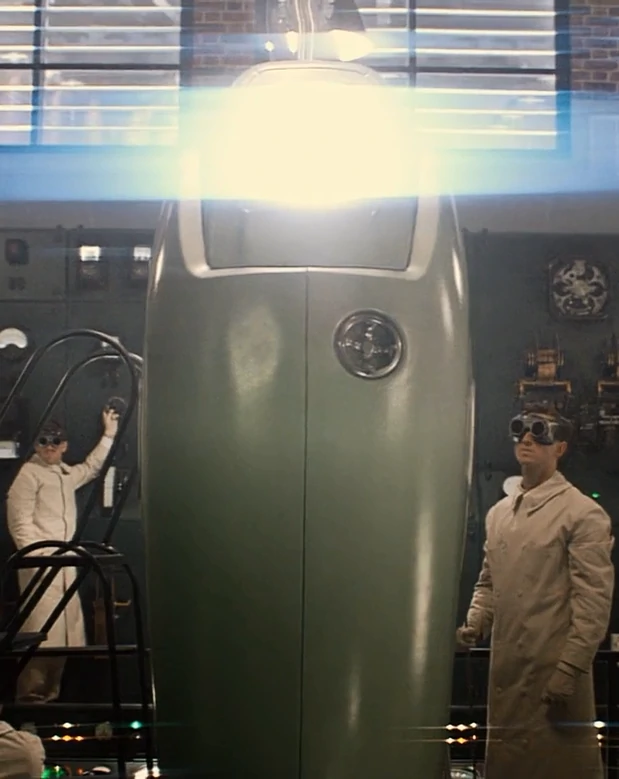
\includegraphics[width=0.5\columnwidth]{Vita_Radiation.png}
\end{center}
\caption{The Model 8086 ``Hero-maker'' issuing low dose vita-ray exposure to a single subject. All subjects were exposed with the same machine for the same length of time and dose. From \citep{vitaradiation}.}
\end{figure}

\section{Results}
Results, in the form of figures, plots or tables, go here. You can leave them in the text or collect them at the end of the manuscript – either is OK for this assignment.  Every figure or table should be numbered and should have a descriptive comment.  All graphs should have well labeled axes with scales and units.  Photos and drawings should also have an indication of scale.  All tables must have sensible units, etc.  You may wish to include summary statistics as a table or on plots.  Indicate the ranges of measurements or the results of statistical testing.  Where applicable, use color coding to help communicate your findings. 

\section{Discussion}
We did not observe any difference reaction times between the group receiving the vita-ray treatment and the placebo group (Figure x, y and z; Table a, b, c; p = 0.547)… These results mean…

Previous studies may have… in contrast, our study… 

Our study did not measure the physical strength or mental status of subjects receiving the treatment.  This could be the subject of future work…

%\section{Conclusions}
%Blah blah…

\section{Acknowledgements}
We thank Dr.~Charles Xavier for advice during data collection and for helpful comments on the manuscript.  We also thank C.~Kent and P.~Parker for their comments on our manuscript.  This work was funded by grants from NIH, DARPA, and the Army Research Lab.    

%\section*{References}
%Please provide references here in alphabetical order and in a biology journal format. 
\bibliography{vitaray.bib}
\end{document}